\subsection{Flight screens}\label{subsec:flight-screens}
\textbf{Flights screen} (Figure \ref{fig:flights}) is for displaying list of the flights.
This screen contains a flight statistics and allows finding certain flights by chosen filters.
By the every flight, it shows its state in case it is planned and current flight.
In addition, it contains the button for export the whole flight history.
If a user choose planned flight, it shows to him the Flight plan screen, what is planned flight summary - it consists of various parameters.
For finnished flight is possible to show \textbf{Flight detail} and for current flight \textbf{In-flight detail}.

\textbf{Flight detail screen} (Figure \ref{fig:flight_detail}) contains all information about a flight including the option to play flight track from start to the end.
\textbf{In-flight detail screen} (Figure \ref{fig:in_flight}) contains information about the flight in real time.
Thanks to \textbf{sliding up panel} (Figure \ref{fig:in_flight_pulled_up}) we can see more information and still check if a drone did not escape the reservation area.

\textbf{Plan a flight} is a group of three screens that represent a wizard for flight plan.
In the first screen (Figure \ref{fig:plan_a_flight_1}), user sets identification properties and planned time of flight.
In the second screen (Figure \ref{fig:plan_a_flight_2}), user sets a polygon for planned flight and its maximum altitude.
In the last screen (Figure \ref{fig:plan_a_flight_3}), user confirms set parameters of planned flight.
It is like a summary.


\begin{figure}
    \centering
    \begin{minipage}{.45\textwidth}
        \centering
        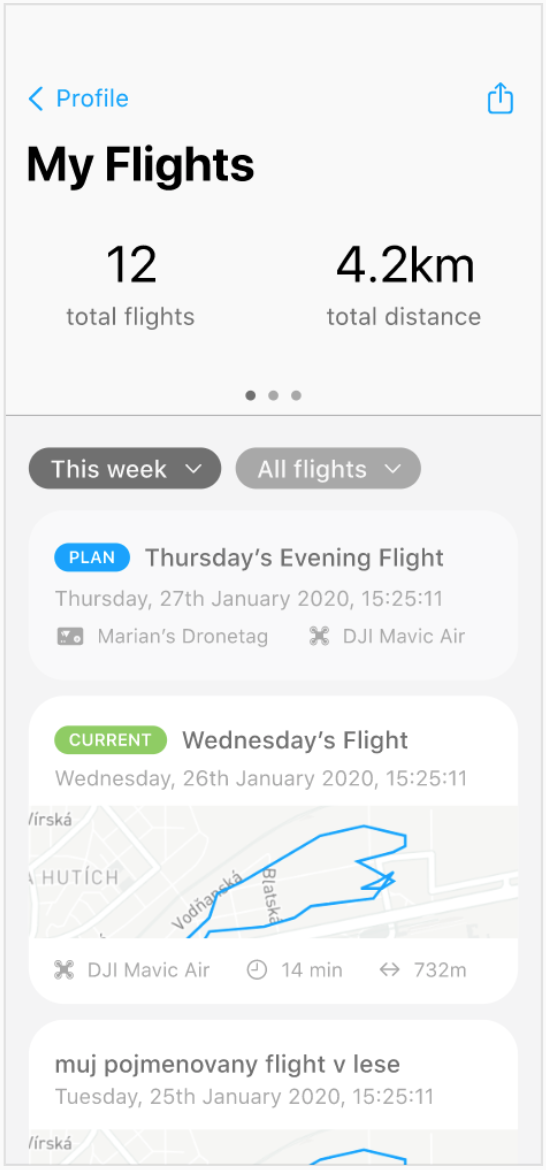
\includegraphics[width=.7\linewidth]{assets/user_interface_design/flight/flights.png}
        \caption{[A50] Flights}
        \label{fig:flights}
    \end{minipage}%
    \hspace{.05\linewidth}
    \begin{minipage}{.45\textwidth}
        \centering
        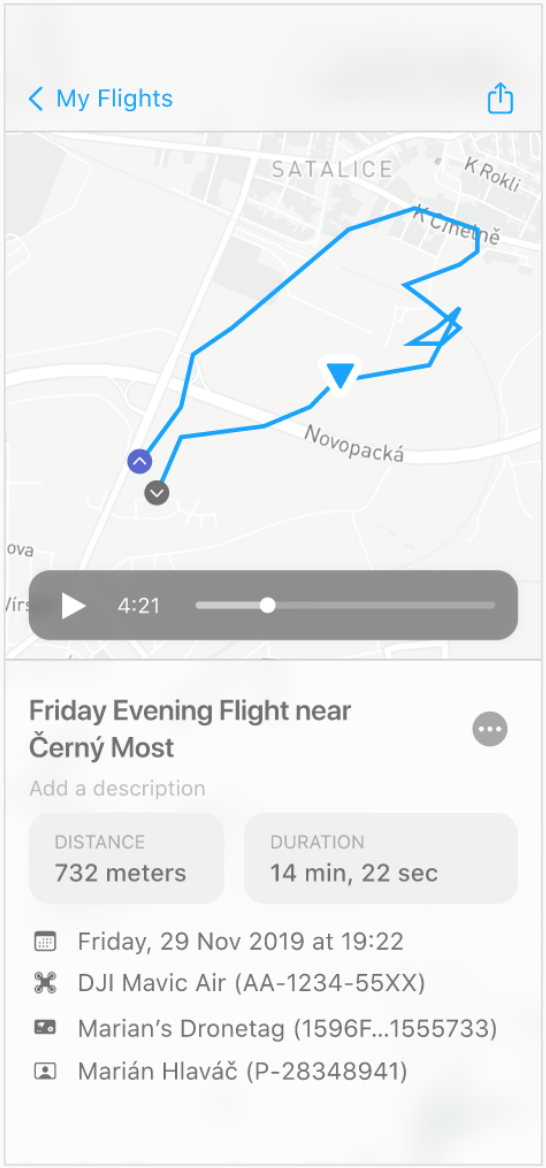
\includegraphics[width=.7\linewidth]{assets/user_interface_design/flight/flight_detail.png}
        \caption{[A51] Flight Detail}
        \label{fig:flight_detail}
    \end{minipage}
    \label{fig:flight_all}
\end{figure}

\begin{figure}
    \centering
    \begin{minipage}{.45\textwidth}
        \centering
        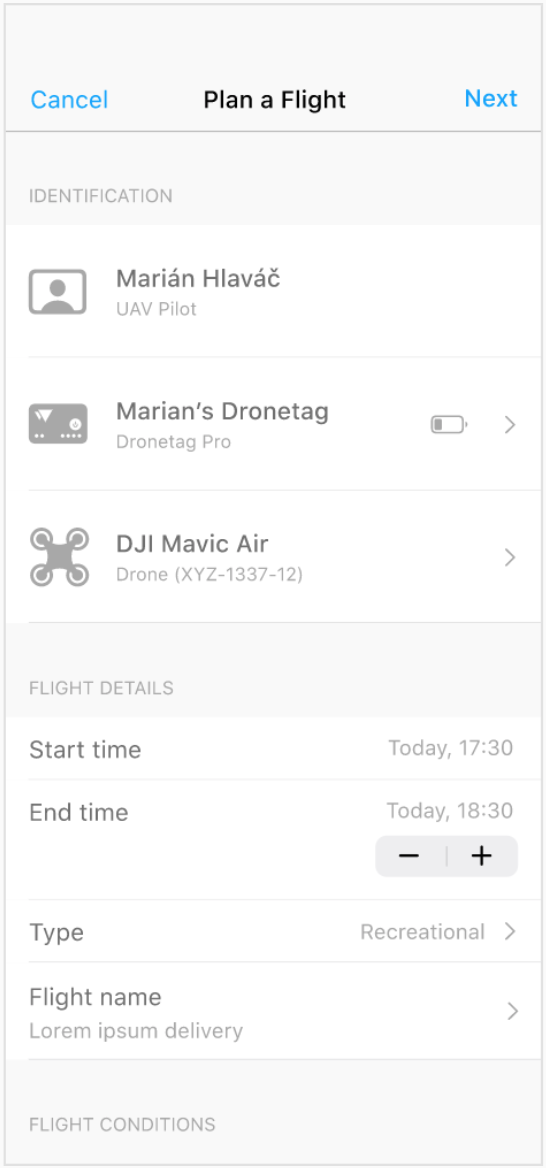
\includegraphics[width=.7\linewidth]{assets/user_interface_design/flight/plan_a_flight_step_1.png}
        \caption{[A33] Plan a Flight - Step 1}
        \label{fig:plan_a_flight_1}
    \end{minipage}%
    \hspace{.05\linewidth}
    \begin{minipage}{.45\textwidth}
        \centering
        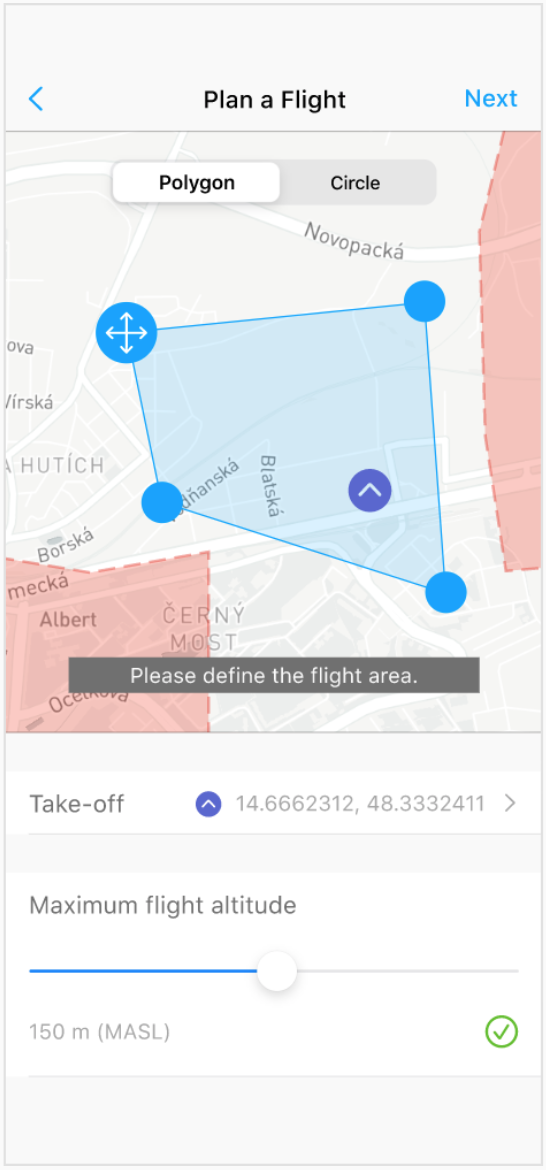
\includegraphics[width=.7\linewidth]{assets/user_interface_design/flight/plan_a_flight_step_2.png}
        \caption{[A34] Plan a Flight - Step 2}
        \label{fig:plan_a_flight_2}
    \end{minipage}
    \label{fig:plan_a_flight_all}
\end{figure}

\begin{figure}
    \centering
    \begin{minipage}{.45\textwidth}
        \centering
        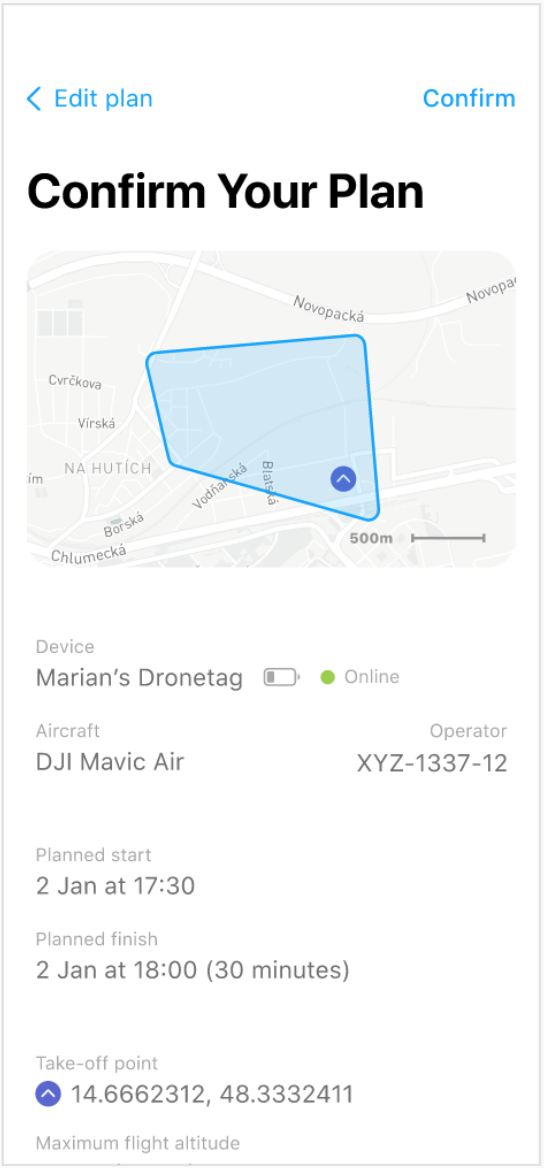
\includegraphics[width=.7\linewidth]{assets/user_interface_design/flight/plan_a_flight_step_3.png}
        \caption{[A35] Plan a Flight - Step 3}
        \label{fig:plan_a_flight_3}
    \end{minipage}%
    \hspace{.05\linewidth}
    \begin{minipage}{.45\textwidth}
        \centering
        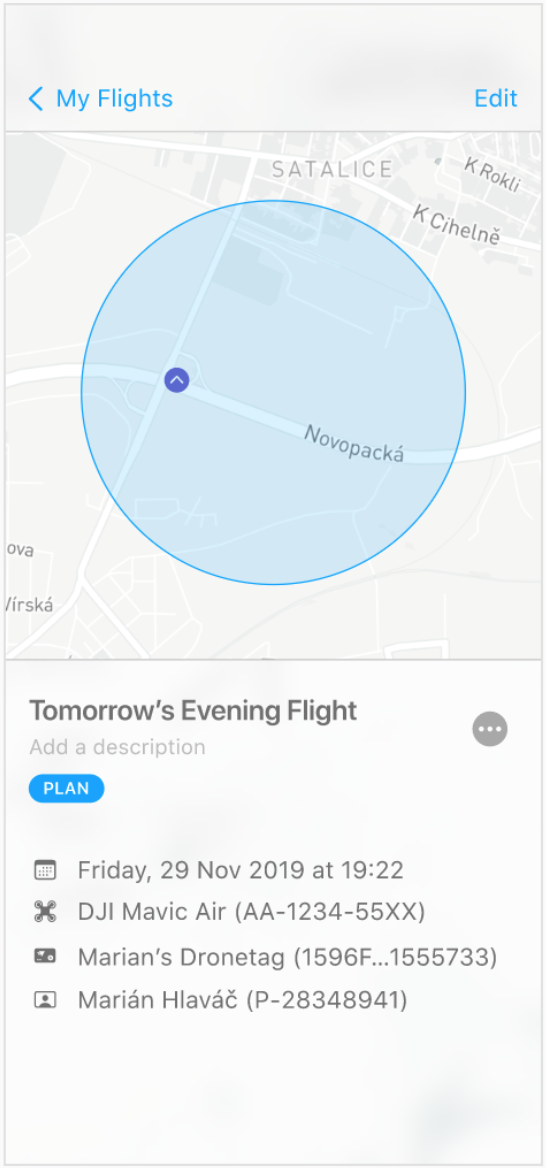
\includegraphics[width=.7\linewidth]{assets/user_interface_design/flight/flight_plan.png}
        \caption{[A52] Flight plan}
        \label{fig:flight_plan}
    \end{minipage}
    \label{fig:plan_a_flight_all_2}
\end{figure}

\begin{figure}
    \centering
    \begin{minipage}{.45\textwidth}
        \centering
        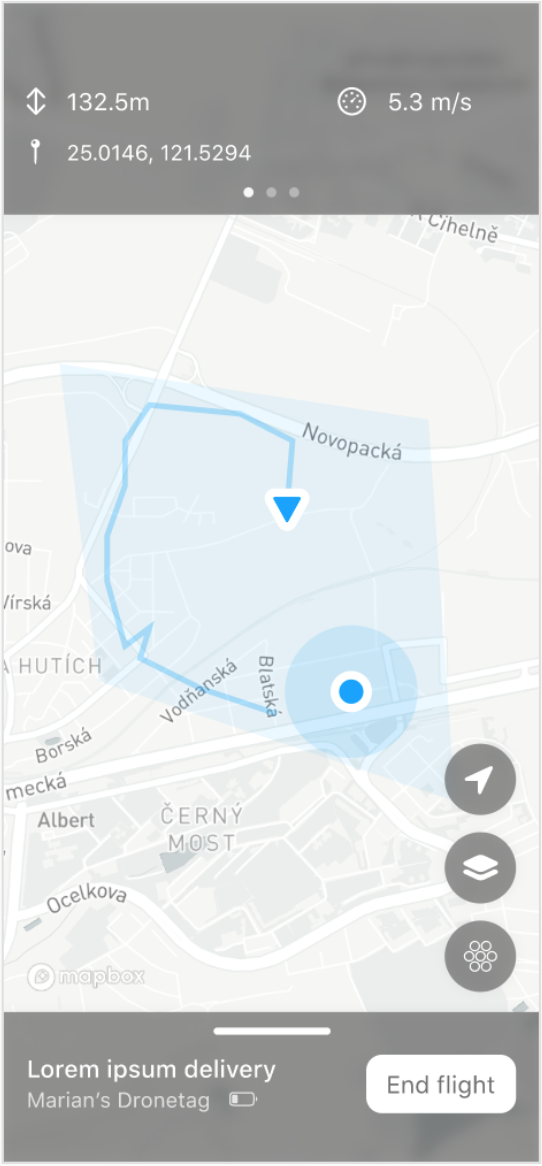
\includegraphics[width=.7\linewidth]{assets/user_interface_design/flight/in_flight.png}
        \caption{[A30] In-Flight}
        \label{fig:in_flight}
    \end{minipage}%
    \hspace{.05\linewidth}
    \begin{minipage}{.45\textwidth}
        \centering
        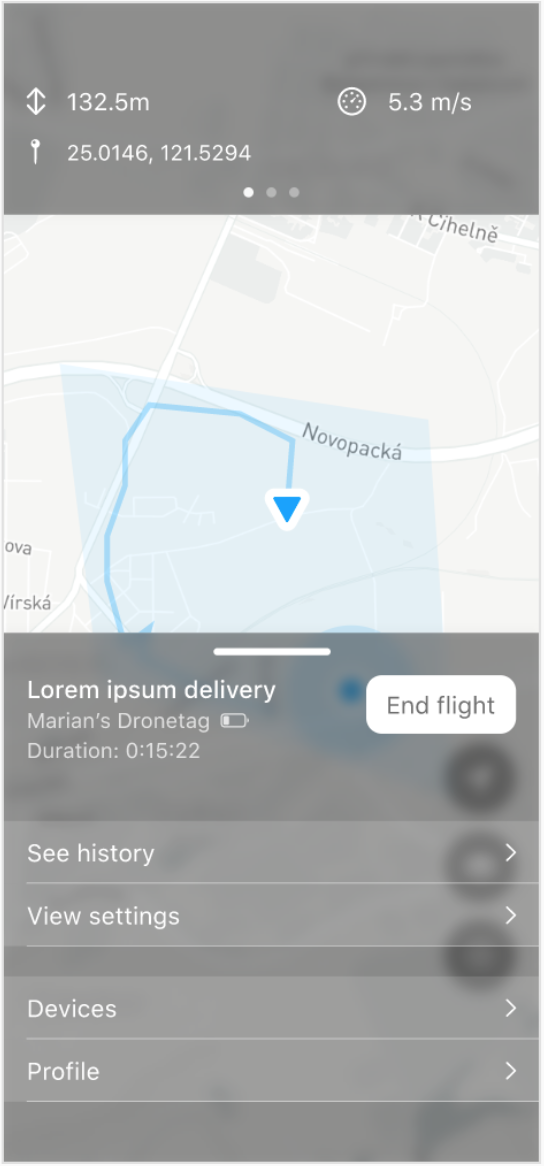
\includegraphics[width=.7\linewidth]{assets/user_interface_design/flight/in_flight_pulled_up.png}
        \caption{[A31] In-Flight, Pulled up}
        \label{fig:in_flight_pulled_up}
    \end{minipage}
    \label{fig:in_flight_all}
\end{figure}

